\section{Funktionale Anforderungen}



- Einleitender Satz
- Unterteilung der Anwender in:
	- Gastgeber ist Admin
	- Gast ist Party People

\subsection{Anwendungsfälle}

Party People:
Möchte Playlist und Current Song einsehen können.
Kann Songs innerhalb der Playlist voten.
Kann seinen DI zurück melden
Möchte Verlauf seines DIs abrufen können
Möchte seine bisherigen Votings abrufen können
Admin:
Verwaltet globale Song Liste
Kann eine Party starten und beenden

\begin{figure}
\centering
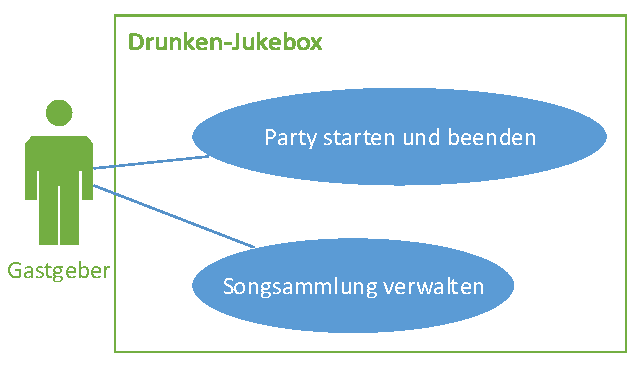
\includegraphics[width=0.75\linewidth]{Bilder/AdminUseCase}
\caption{}
\label{fig:AdminUseCase}
\end{figure}

\begin{figure}
\centering
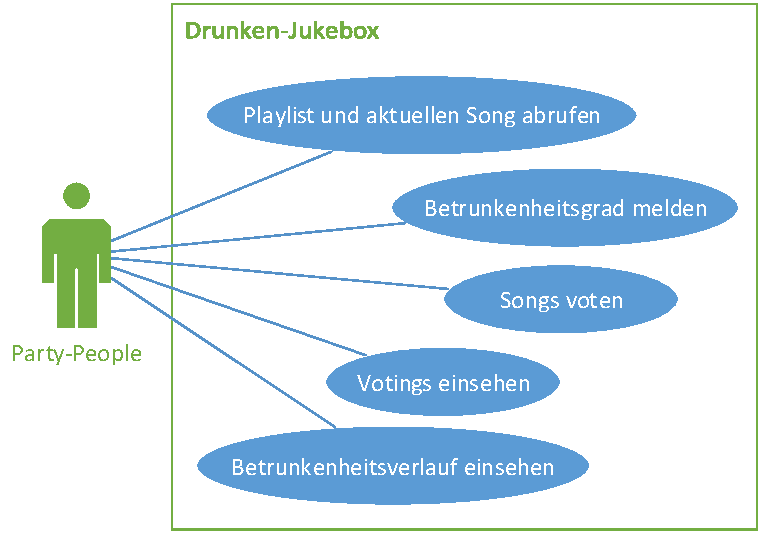
\includegraphics[width=0.95\linewidth]{Bilder/PartyPeopleUseCase}
\caption{}
\label{fig:PartyPeopleUseCase}
\end{figure}
